%%%%%%%%%%%%%%%%%%%%%%%%%%%%%%%%%%%%%%%%%%%%%%%%%%%%%%%%%%%%%%%%%%%%%%
% How to use writeLaTeX: 
%
% You edit the source code here on the left, and the preview on the
% right shows you the result within a few seconds.
%
% Bookmark this page and share the URL with your co-authors. They can
% edit at the same time!
%
% You can upload figures, bibliographies, custom classes and
% styles using the files menu.
%
%%%%%%%%%%%%%%%%%%%%%%%%%%%%%%%%%%%%%%%%%%%%%%%%%%%%%%%%%%%%%%%%%%%%%%

\documentclass[14pt]{article}

\usepackage{sbc-template}

\usepackage{graphicx,url}

\usepackage[brazil]{babel}   
\usepackage[utf8]{inputenc}  

\usepackage{fancyhdr}
\usepackage{amsmath}
\usepackage{verbatim}
\pagestyle{fancy}

\fancyhead[L]{ }
\fancyhead[R]{ }
\renewcommand{\headrulewidth}{0pt}
\sloppy
\begin{document} 



\title{Classe de problemas P, NP e NP-Completos}

\author{Diogo O. Neiss}
  

\address{Graduandos em Ciência da Computação \\
Pontifícia Universidade Católica de Minas Gerais
(PUC MG)\\
Av. Dom José Gaspar, 500 Coração Eucarístico - Belo Horizonte - MG 30535-901, Brasil\\
\email{diogo.neiss@sga.pucminas.br}
}

\maketitle
     
%\section*{Introdução} \label{sec:firstpage}

  Um problema dito como "P", isto é, de solução polinomial, é um problema que pode ser resolvido através de um algoritmo x, tal que x tenha sua complexidade como uma função         polinomial, como $n^{3} + 5n^{2}+3n$. Por exemplo, o algoritmo de ordenação bubble sort possui complexidade $O(n^2)$ , enquanto o algoritmo de Held-Carp (relacionado ao problema do caixeiro viajante, que é NP, isto é, Tempo Polinomial não determinístico) possui complexidade $O({2^{n}} * n^{1/2})$. Abaixo, podemos ver a imensa diferença quando x aumenta de tamanho. 
  \begin{figure}[h]
      \centering
      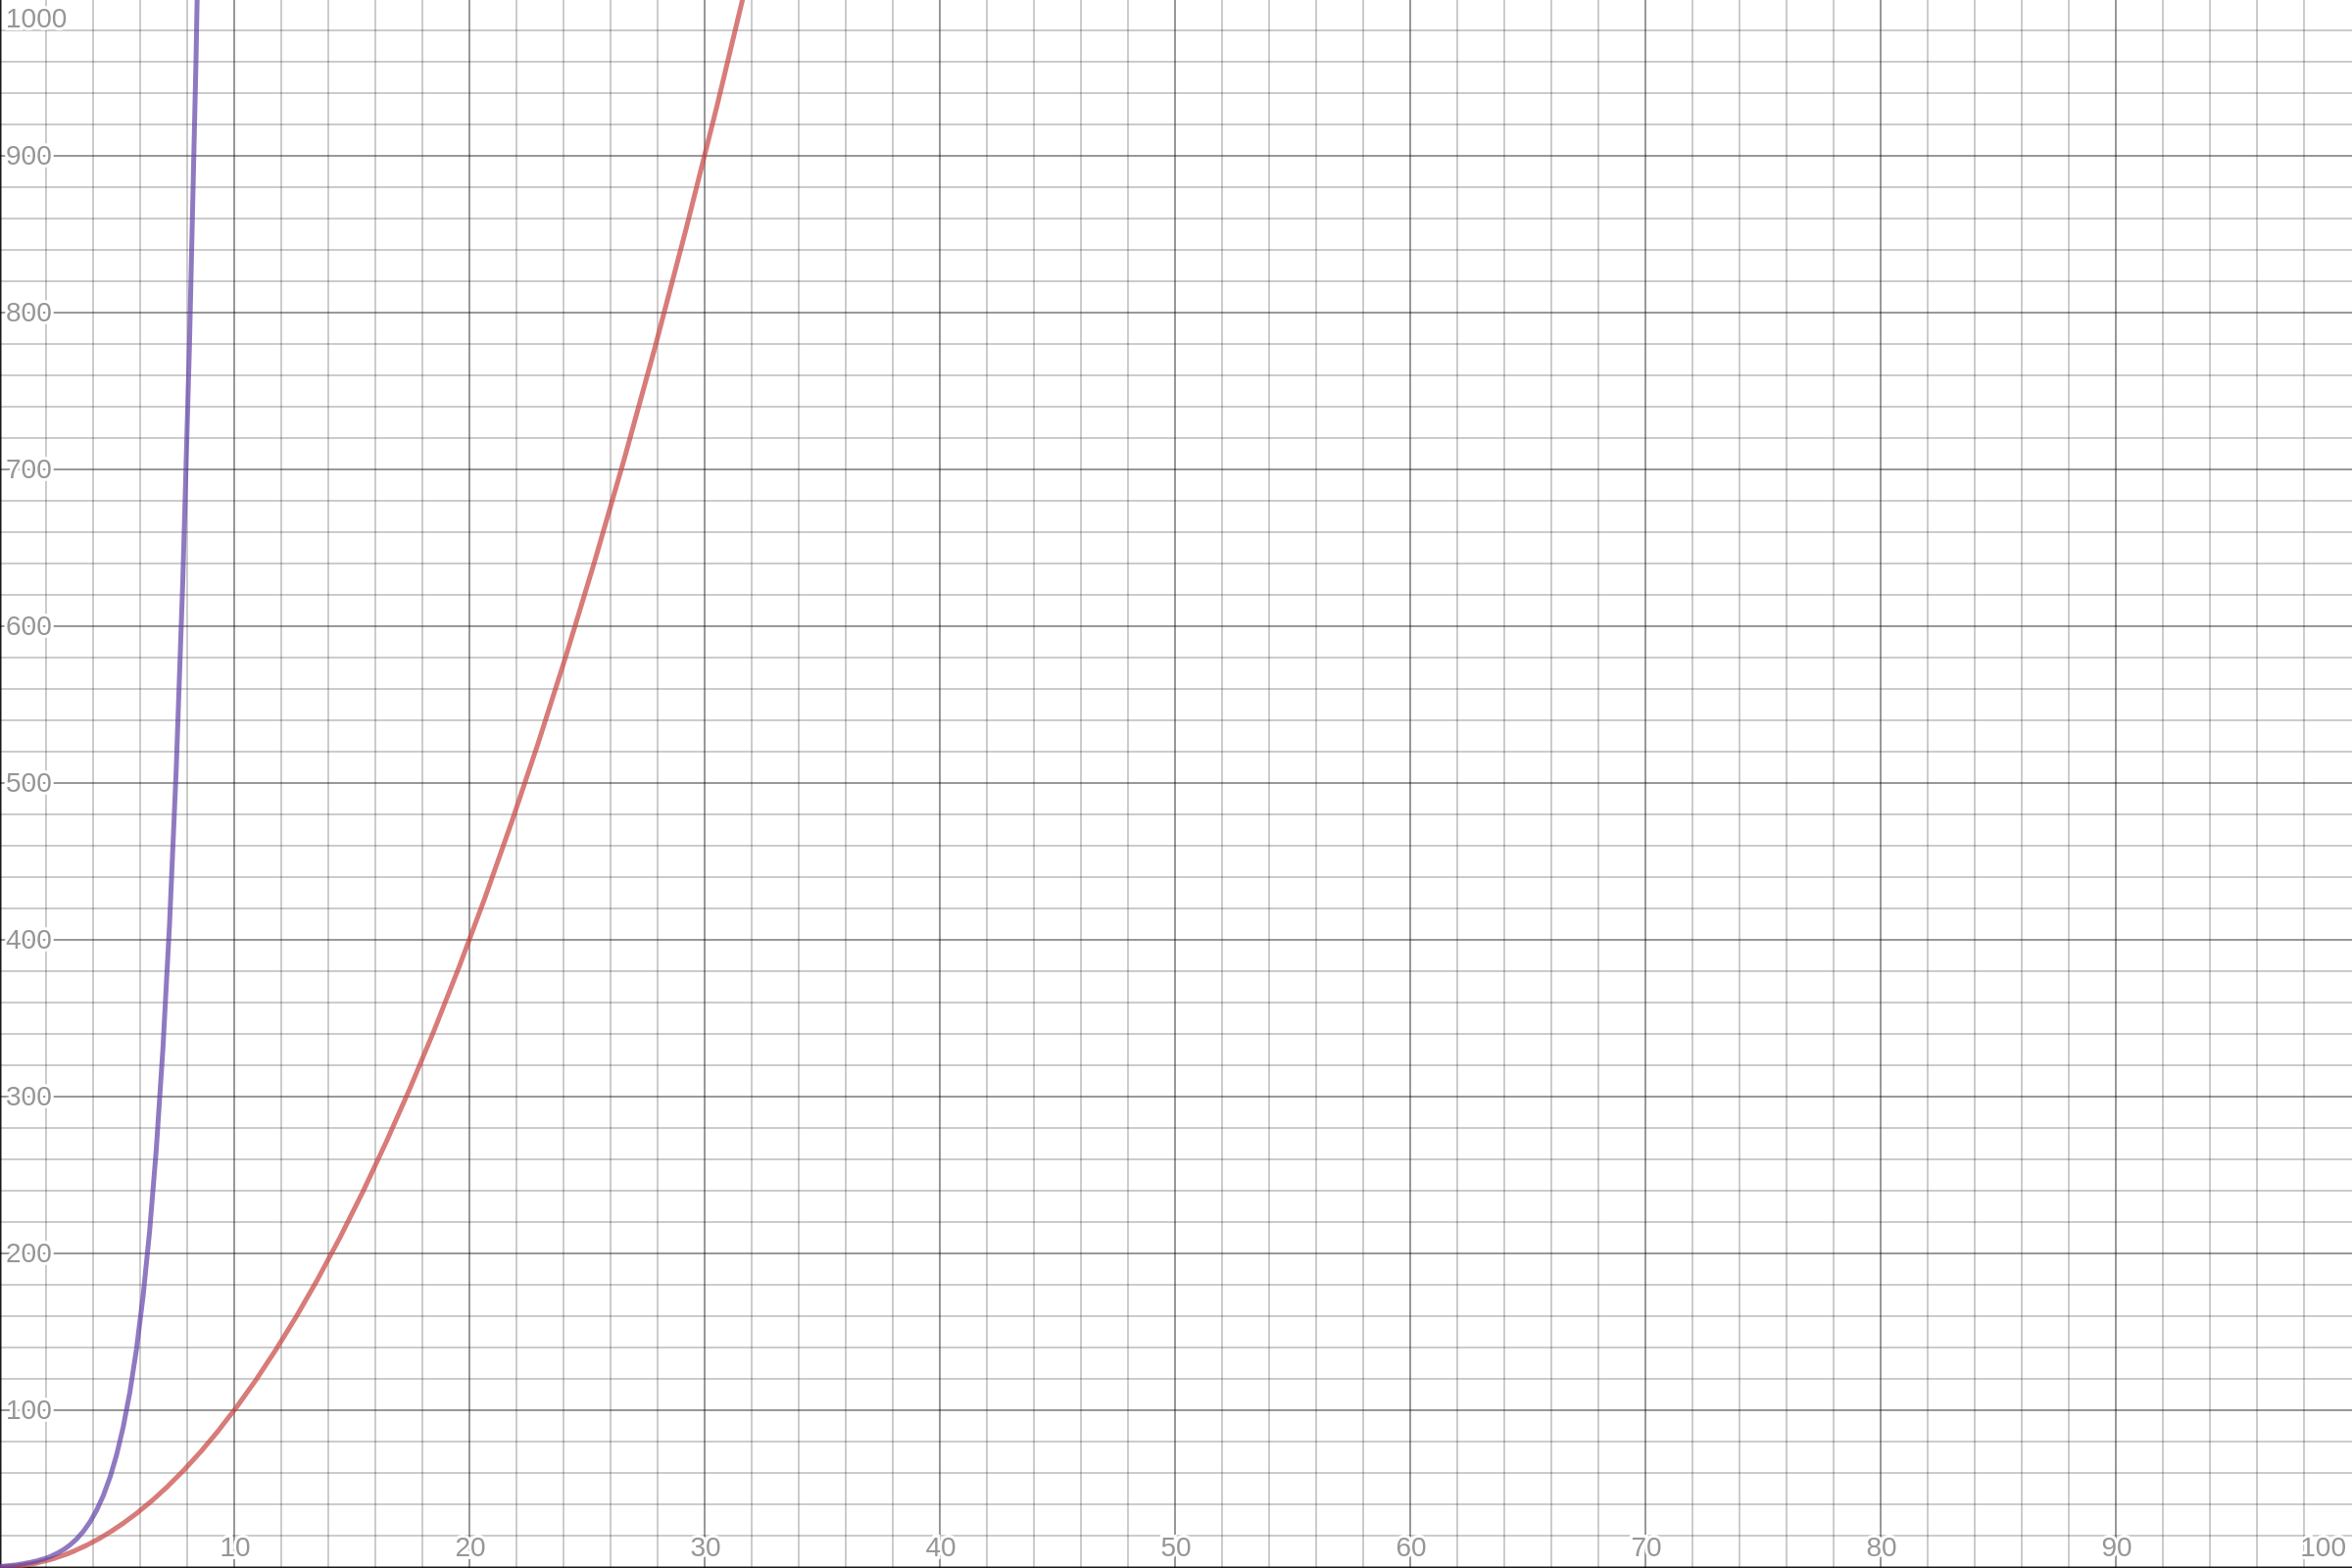
\includegraphics[width=6cm]{desmos-graph.png}
      \caption{\textit{f(x)} da complexidade do bubble sort, em vermelho, e do algoritmo de Held-Carp, em roxo.}
      \label{fig:grafico}
  \end{figure}
  
Há problemas onde \textit{não são conhecidos} algoritmos eficientes
para resolvê-los. Eles são chamados de problemas N P-completos. Até a presente data provar que \textit{P = NP} ou que \textit{P != NP} permanece como um dos notórios problemas do milênio.

Problemas NP-Completos tem a característica notavel de que se um deles admitir um algoritmo “eficiente” então todos admitem algoritmos “eficientes”, ou seja, resolver um problema nesta classe ocasiona na solução de diversos outros, uma vez que estão na mesma classe. \cite{UFPR:Vignatti}

Uma propriedade interessante dos problemas NP é a dificuldade de se encontrar uma solução em contraste com a verificação. Por exemplo, descobrir os fatores primos que compõe o primo 269 é razoavelmente rápido, uma vez que é pequeno, com a verificação de acerto custando uma única operação, dividir o número pelos fatores encontrados. Conforme o tamanho do primo aumenta o tempo de cálculo de seus fatores aumenta absurdamente, com o tempo de verificação constante, de uma operação. Portanto, conclui-se que verificar a solução de um problema NP é polinomial \cite{kleinberg:2006}

Por fim, uma curiosidade interessante: a própria prova de P = NP é um problema NP-Completo, uma vez que é extremamente complexo formular um teorema acerca disso, com a verificação de que o teorema está correto sendo verificável em tempo polinomial.
  
Caso resolvido, o "Clay Mathematics Institute" propõe um prêmio de US\$1.000.000, como solução de um dos 7 problemas do milênio. Os impactos positivos, caso seja provada uma possível solução P para a classe de problemas NP, seriam imensuráveis, indo desde \textit{Suduko} até combate ao câncer, através de algoritmos melhores para \textit{protein folding}.





%\section*{Aplicações}

\bibliographystyle{sbc}
\bibliography{sbc-template}

\end{document}
